\settitle[CorkaMIX]{CorkaMIX : polyglottes binaires et implications}


\setauthor[M.~Albertini]{Ange Albertini\\
  \email{ange.albertini@gmail.com}}
\institute{Corkami.com}


\maketitle
\index{Ange, M.}

\begin{abstract}
De l'exploitation à l'infection, les {\it malwares} modernes utilisent de nombreux formats de fichier binaires.
Il est crucial de pouvoir correctement les identifier et les analyser, si possible de manière automatique.
À priori clairement différenciés, il est malheureusement possible de combiner certains d'entre eux dans un seul et même fichier.
De tels binaires {\it polyglottes} ont donc dans un premier temps été crée. 
Ensuite, plusieurs caractéristiques non documentées de chaque format concerné ont été rajoutées, pour mettre en évidence l'importance du problème entre les limites des documentations officielles, et la réalité (du monde des virus).
Les conséquences sur le fonctionnement des outils de sécurités sont finalement mises en évidence, avec ce que ça implique pour l'utilisateur final.
\end{abstract}


\section{Introduction}

\subsection{État de l'art}

Un fichier polyglotte est un seul et meme fichier fonctionnant comme on s'y attend avec plusieurs languages différents.  Un des plus simple d'entre eux, représenté par le Polyglot de David Kendall figure~\ref{lst:albertini:polyglot}, fonctionne en Ruby, Perl, PHP, ksh, Scheme, Lisp, Clojure, Plan. Les {\it polyglottes} peuvent aller beaucoup plus loin, jouant sur les différences d'interprétation et de {\it pré-processing} de chaque language inclu.

\begin{lstlisting}[language={},caption={un programme polyglotte simple},label={lst:albertini:polyglot}]
 (print "Hello, world!\n");
\end{lstlisting}
Cependant, les formats de fichiers binaires sont, eux, rarement compatibles, car exclusifs: en effet, la majeure partie d'entre eux doivent nécessairement débuter par une {\it signature} dite 'nombre magique', à chaque fois différente, à de rares exceptions près (tel {\em CAFEBABE}, pour le format Mach-O universel et les classes JAVA).

Il ne semble donc pas possible de combiner des formats binaires en général. Cependant, il y a quelques exceptions. Et hélàs - ce n'est pas une coincidence - il s'agit des formats parmi les plus utilisés ces dernières années pour la prolifération de {\it malware}.

\subsection{Pivot}

Le format pivot de la grande majeure partie des virus est le format de binaire universel de Windows, appelé le format {\it Portable Executable}, ou {\em PE}. Pour ce rôle unique dans la chaîne virale, il a donc été choisi comme point de départ.

\section{exploration du format {\em PE}}
Ce format stipule que le fichier commence par une structure {\em IMAGE\_DOS\_HEADER}, de 40 octets:
\begin{itemize}
\item les 2 premiers octets de cette structure, appelé {\em e\_magic}, contiennent obligatoirement la signature {\em MZ} (bien que le vieux format d'exécutable DOS tolérait officieusement les lettres {\em ZM} - probablement à titre comique - ce n'est plus le cas pour les fichiers {\em PE}. Il est donc impossible de le combiner à tout autre format imposant une signature spécifique à l'octet 0.
\item tous les champs suivants, à l'exception du dernier, ne concerne que la fonctionnalité DOS de l'exécutable - qui se borne en majeure partie à afficher un message d'erreur, elle est totalement ignorée quand le fichier est chargé en tant que {\em PE}.
\item le dernier champ, {\em e\_lfanew}, est un pointeur sur 32 bits vers la structure suivante de l'exécutable
\end{itemize}

On sait donc que notre fichier doit commencer par {\em M} et {\em Z}, et qu'au déplacement $0x3C$ doit se trouver un pointeur. Entre les deux, on peut y faire ce que l'on veut, tout en gardant la fonctionalité {\em PE} intacte.

C'est ce que nous allons faire en y intégrant un script Python.

\subsection{intégration d'un script Python}

un script Python est un fichier texte qui commence à l'octet 0. les 2 premières lettres étant imposées, il faut donc utiliser ce {\em MZ} en créant, par exemple, une variable fictive.
\begin{lstlisting}[language={Python},caption={un script python commençant par MZ},label={lst:albertini:pythonMZ}]
MZ=1
\end{lstlisting}

Mais l'interpréteur Python vérifie à l'avance l'encodage de tout le fichier source. Sachant que la structure suivante, pointée par {\em e\_lfanew}, {\em IMAGE\_NT\_HEADERS} a comme premier champ {\em Signature} qui doit contenir les caractères nuls, on se trouve face à un obstacle.

Il est néanmoins facile à contourner, il suffit d'insérer entre le déplacement 0 et cette {\em Signature} un caractère de fin de fichier, {\em EOF}, dont le code est 26.

On a aussi la place d'insérer une partie de script Python fonctionnelle, histoire de prouver que ça marche effectivement.
Le python ne permettant pas lui-même de générer un caractère de fin de fichier dans son propre source (sans quoi, logiquement, le fichier sera tronqué), le fichier sera nécessairement dorénavant généré en assembleur.
\begin{lstlisting}[language={},caption={un script python généré en assembleur},label={lst:albertini:pythonasm}]
db 'MZ=1;print("Hello World !")'
db 26 ; EOF
\end{lstlisting}

Ça peut se faire avec n'importe quel exécutable, en écrasant l'obsolète {\em IMAGE\_DOS\_HEADER}, à l'exception de sa signature et du dernier champ {\em e\_lfanew}, comme montré à la figure~\ref{fig:albertini:pythonnotepad}.
\begin{figure}[ht]
  \centering
  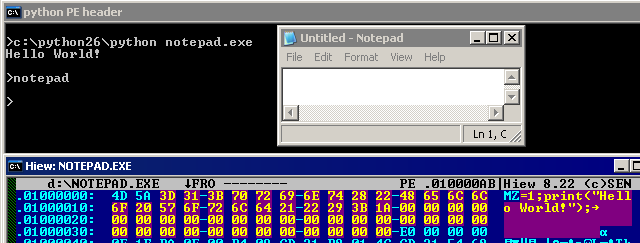
\includegraphics[width=0.8\textwidth]{albertini/img/pythonnotepad}
  \caption{le bloc-note Windows avec un en-tête Python}
  \label{fig:albertini:pythonnotepad}
\end{figure}

\subsection{création d'une page HTML dans un exécutable}

Le laxisme omniprésent dans les pages HTML fait qu'au final, les navigateurs se contente d'ignorer un peu tout, quand bien même ce serait du binaire pure, au cas où un tag $<HTML>$ finirait par être présent.

Ansi, le simple fait de rajouter à la fin d'un exécutable du code HTML va en faire une page web fonctionnelle, pour peu qu'on renomme l'extension du fichier, comme le montre la figure~\ref{fig:albertini:htmlnotepad}.

\begin{figure}[ht]
  \centering
  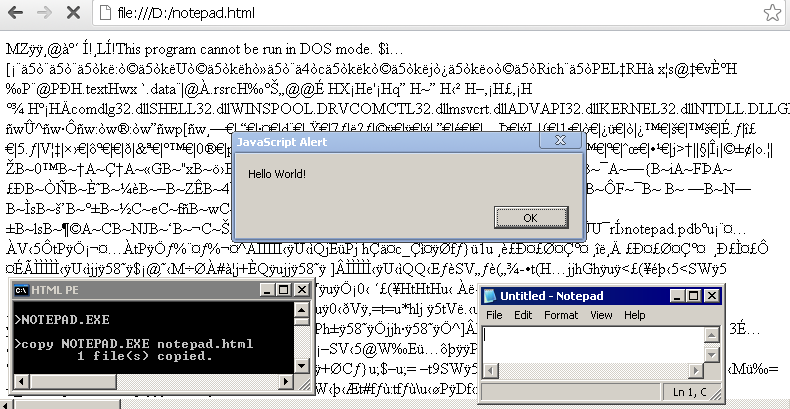
\includegraphics[width=0.8\textwidth]{albertini/img/htmlnotepad}
  \caption{le bloc-note Windows avec une page HTML ajoutée à la fin}
  \label{fig:albertini:htmlnotepad}
\end{figure}

parasites visuels dûs aux binaire~$\Rightarrow$~jouer sur les CSS pour rendre le code invisible

rajouter quelque chose après la page HTML~$\Rightarrow$~ouverture d'un bloc de commentaire non fermé

\subsection{concaténation d'un PDF et d'un exécutable}

La documentation officielle d'Adobe stipule que la première ligne d'un PDF doit être sa signature.

\begin{figure}[ht]
  \centering
  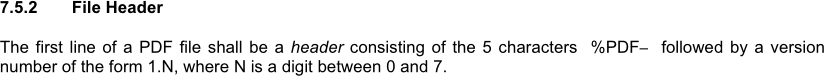
\includegraphics[width=0.8\textwidth]{albertini/img/pdfsigtheory}
  \caption{Documentation officielle imposant la signature d'un PDF à la première ligne}
  \label{fig:albertini:pdfsigtheory}
\end{figure}

En pratique, il n'en n'est rien, il est juste requis qu'une signature valide soit présente dans les 1024 ($0x400$) premiers octets.

\begin{figure}[ht]
  \centering
  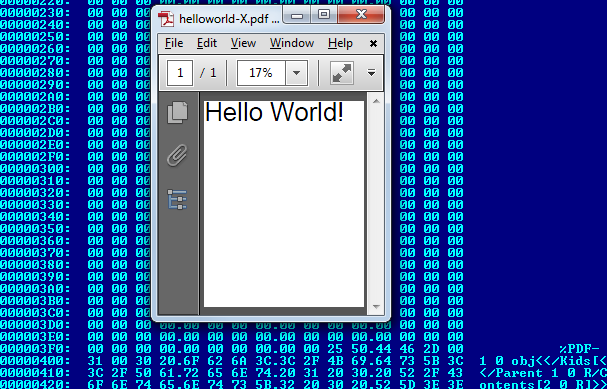
\includegraphics[width=0.8\textwidth]{albertini/img/pdfsigpractice}
  \caption{un PDF reconnu par Adobe dont la signature est à la fin des 1024 premiers octets}
  \label{fig:albertini:pdfsigpractice}
\end{figure}

On peut donc, dans un premier temps, rajouter à la fin d'un petit exécutable un PDF dans son intégralité, et les 2 fonctionneront encore comme on s'y attend.

\begin{figure}[ht]
  \centering
  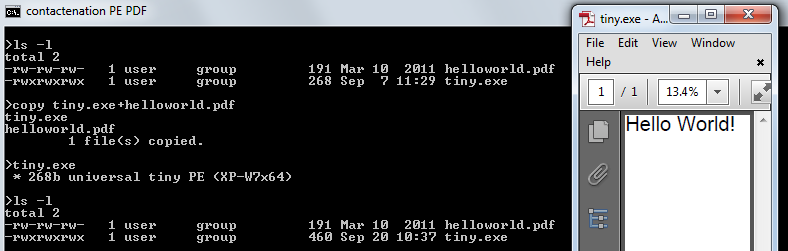
\includegraphics[width=0.8\textwidth]{albertini/img/tinyPEPDF}
  \caption{un PDF greffé à la fin d'un petit exécutable}
  \label{fig:albertini:tinyPEPDF}
\end{figure}

\begin{itemize}
\item gros PE $\Rightarrow$ rajouter la signature PDF dans l'en-tête PE

\begin{figure}[ht]
  \centering
  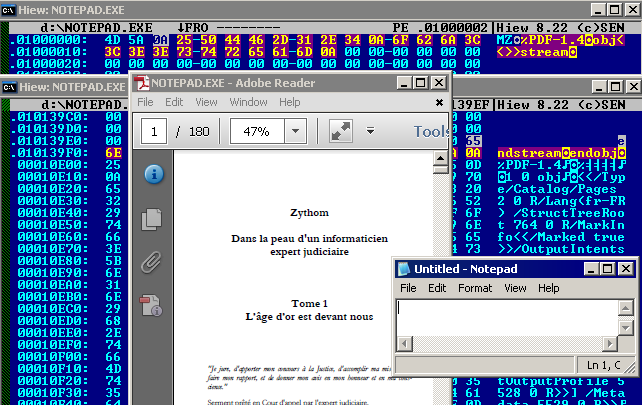
\includegraphics[width=0.8\textwidth]{albertini/img/pdfnotepad}
  \caption{le bloc-note Windows avec un fichier PDF ajouté à la fin}
  \label{fig:albertini:pythonnotepad}
\end{figure}


\item eviter le contenu du PE d'être interprété $\Rightarrow$ créer un objet PDF fictif
\end{itemize}

\subsection{un ZIP dans un exécutable}
le format ZIP n'impose rien quant au début du fichier.
en revanche, il doit terminer strictement le fichier.

un JAR n'est qu'une archive pour une ou plusieurs classes Java (extension .CLASS), et d'un $manifest$.

si on rajoute un seul octet à la fin d'un Zip utilisé comme JAR, Java ne reconnait plus ce fichier comme valide.

Au contraire, si l'interpreteur python détecte la présence d'un ZIP, il va traiter le fichier comme un {\em python egg}, donc n'interprétera plus le fichier à son début comme un script.

le format .JAR et .PY sont donc exclusivement opposés.


\subsection{recapitulons}
\begin{itemize}
\item un PE
\item une signature PDF dans ses $1024 - 6$ premier octets
\item concaténer le PDF au PE
\item concaténer la page HTML
\item concaténer le ZIP
\end{itemize}

\section{compliquons un peu}
faisons tout à la main, pour garder le contrôle.

toutes les structures crées à partir de zéro, en assembleur.

un fichier Zip sans compression stocke le fichier original tel quel, ce qui nous permet de générer le fichier zippé sans la moindre retouche nécessaire.

\subsection{un PE fait main}
pour avoir un contrôle total de la génération du PE, il est entièrement généré en assembleur, pour son code et ses données bien sûr, mais également pour sa structure complète.

\begin{itemize}
\item peu d'éléments définis

seulement 18 éléments définis dans l'en-tête, toutes structures confondues. par rapport à 40 dans un exécutable $Hello World$ compilé en assembleur standard.
\begin{figure}[ht]
  \centering
  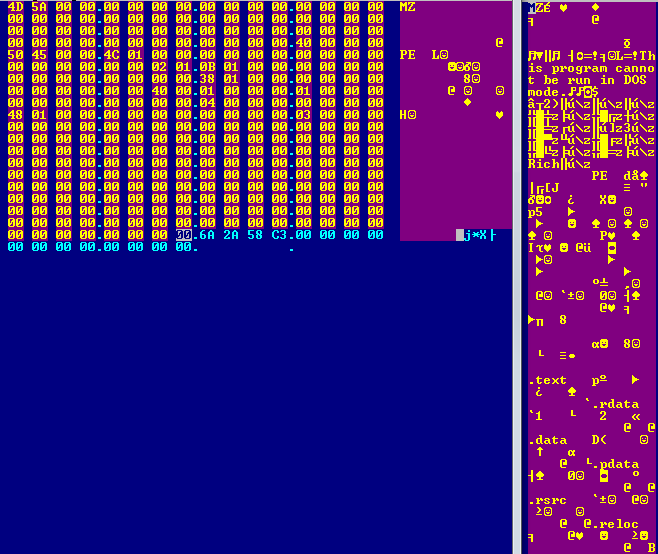
\includegraphics[width=0.8\textwidth]{albertini/img/empty_pe_header}
  \caption{comparaison d'en-têtes PE}
  \label{fig:albertini:empty_pe_header}
\end{figure}

\item pas de sections

Quand un exécutable utilise des alignements faibles, tout l'exécutable est chargé en mémoire indépendamment de la table des sections. il devient dans ce cas possible de ne pas définir de section du tout $NumberOfSections = 0$, et de ne pas avoir de table de section $SizeOfOptionalHeader = 0$

\item du code non documenté

que les assembleurs standards ne peuvent même pas encoder.

{\em SetALC}

{\em nop} multi-octets

absent de la documentation Intel, mais présent dans la documentation AMD.

ça donne des inconnues dans tous les outils Microsoft.
\begin{figure}[ht]
  \centering
  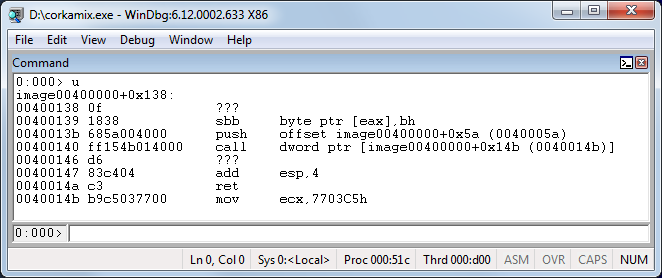
\includegraphics[width=0.8\textwidth]{albertini/img/corkamix_windbg}
  \caption{WinDbg montre plusieurs instructions inconnues}
  \label{fig:albertini:corkamix_windbg}
\end{figure}

\begin{figure}[ht]
  \centering
  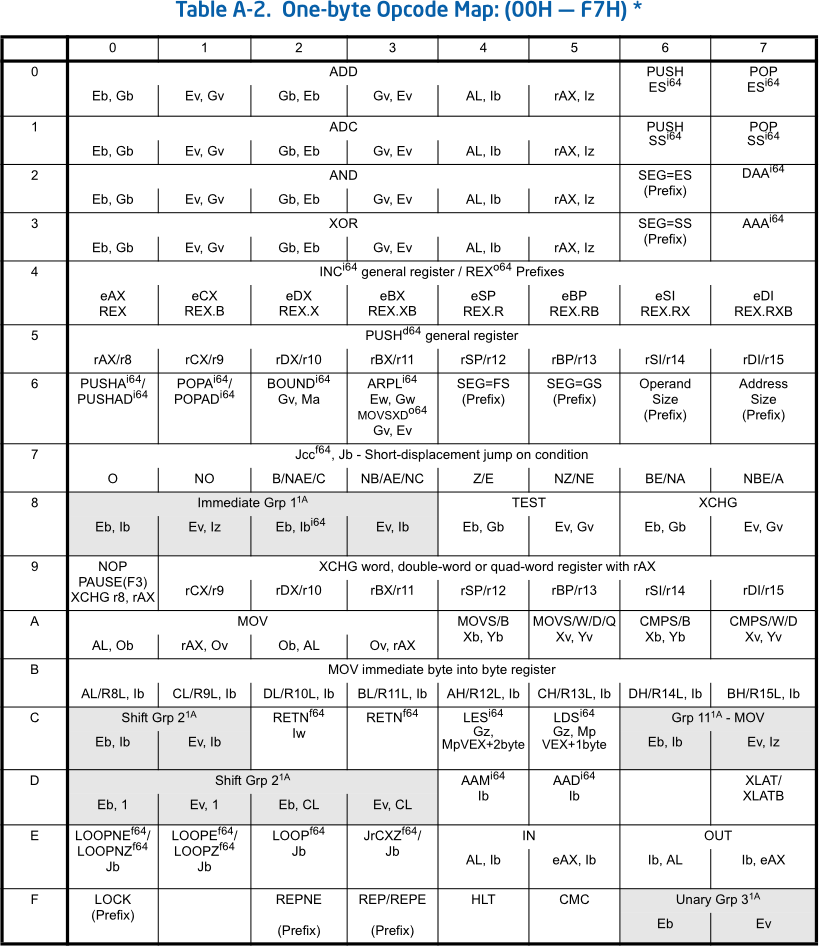
\includegraphics[width=0.8\textwidth]{albertini/img/undoc_setalc}
  \caption{la documentation officielle n'indique rien pour l'octet $D6$}
  \label{fig:albertini:undoc_setalc}
\end{figure}

\begin{figure}[ht]
  \centering
  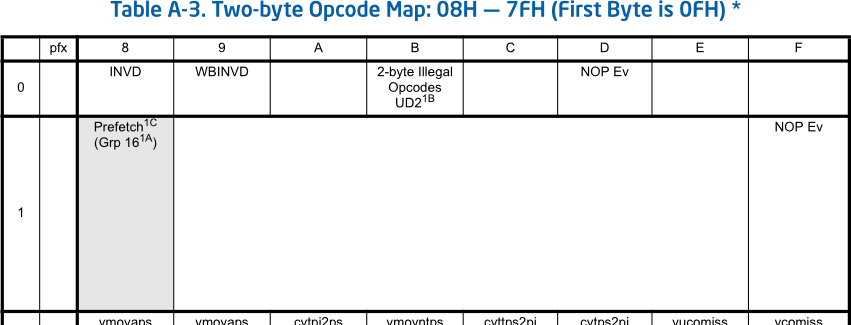
\includegraphics[width=0.8\textwidth]{albertini/img/undoc_nop}
  \caption{la documentation Intel ne mentionne NOP que pour les octets $0F 1F$}
  \label{fig:albertini:undoc_nop}
\end{figure}

\begin{figure}[ht]
  \centering
  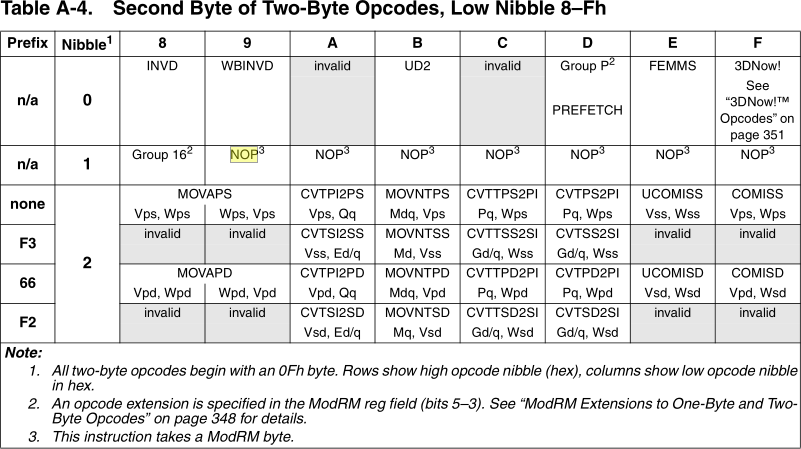
\includegraphics[width=0.8\textwidth]{albertini/img/nop_amd}
  \caption{le NOP de plusieurs octets est complètement documenté par AMD}
  \label{fig:albertini:nop_amd}
\end{figure}


\begin{figure}[ht]
  \centering
  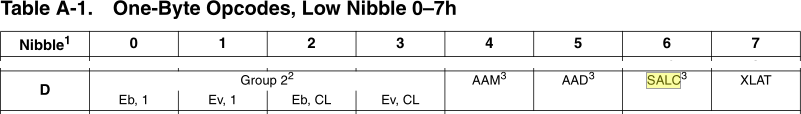
\includegraphics[width=0.8\textwidth]{albertini/img/salc_amd}
  \caption{SetALC est documenté par AMD}
  \label{fig:albertini:salc_amd}
\end{figure}

\item une table d'import très compacte

la liste des descripteur se termine quand Name ou IAT sont nuls.

on intègre l'IAT, très petite, dans le descripteur lui même.

on intègre les noms tronqués de DLL dans le terminateur, ainsi que le ??? hint/name.

une telle structure fortement réduite n'est gérée par aucun outil commercial à l'heure actuelle, Hiew et IDA compris.

\begin{figure}[ht]
  \centering
  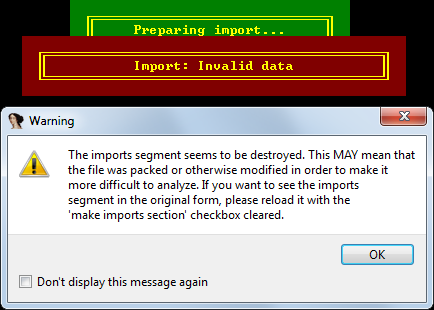
\includegraphics[width=0.5\textwidth]{albertini/img/imports_error}
  \caption{une structure d'imports non gérée par Hiew ou IDA}
  \label{fig:albertini:imports_error}
\end{figure}

ces astuces font que les outils les plus avancés échouent à analyser le PE parfaitement.

\end{itemize}

\subsection{un CLASS Java au régime}
en utilisant le source Java minimal, en supprimant

\begin{lstlisting}[language={java},caption={un Hello World minimal en Java},label={lst:albertini:hwjava}]
 public class HelloWorld
{
  public static void main(String[] args)
  {
    System.out.println("Hello World!");
  }
}
\end{lstlisting}

on obtient un fichier CLASS de 426 octets.
\begin{itemize}
\item 2 méthode dont une superflue
\item un attribut de classe {\em SourceFile} non indispensable
\item les attributs de {\em Code} ont tous un attribut {\em LineNumberTable}, lui non plus non requis.
\end{itemize}

en supprimant toutes les constantes associés à ces éléments non requis, on peut gagner de la place.

Même pour quelque chose d'aussi simple qu'un simple affichage de chaîne, on peut bien réduire le fichier.

en utilisant les options de compilations, on éradique les attributs {\em SourceFile} et {\em LineNumberTable}.

on obtient un fichier de 341 octets.

en utilisant Jasmin, l'assembleur pour Java, on peut réduire le fichier en fusionnant les méthodes et en renommant l'unique restante en 'main', ce qui nous fera de l'espace économisé. En revanche, Jasmin semble toujours rajouter un attribut {\em SourceFile}.

\begin{lstlisting}[language={java},caption={un Hello World minimal en Jasmin},label={lst:albertini:hwjasmin}]
.class public HelloWorld
.super java/lang/Object

.method public static main([Ljava/lang/String;)V
   .limit stack 2   ; up to two items can be pushed

   getstatic java/lang/System/out Ljava/io/PrintStream;
   ldc "Hello World!"
   invokevirtual java/io/PrintStream/println(Ljava/lang/String;)V
   return
.end method
\end{lstlisting}

on se retrouve bloqué, et comme on n'est jamais aussi bien servi que par soit-même, autant tout réécrire en assembleur.
JVM étant basé sur la pile, l'encodage des opérations des très simple. on peut donc le réimplémenter soit-même via des macros.
\begin{lstlisting}[language={java},caption={un Hello World minimal en Java},label={lst:albertini:asmjavamacros}]
%macro GETSTATIC 1
        db 0b2h
            _dw %1
%endmacro

[...]
%macro fieldref 2
        db 9
        _dw %1
        _dw %2
%endmacro
\end{lstlisting}

la structure d'une classe Java n'étant ni compactée ni basé sur des longueurs variables, on peut facilement implémenter un à un chaque champ requis
\begin{lstlisting}[language={java},caption={un Hello World minimal en Java},label={lst:albertini:asmjavafields}]
_dd 0CAFEBABEh ; signature
_dw 3          ; major version
_dw 2dh        ; minor version
[...]
_dw 22        ;constant pool count

; getstatic
  fieldref 9, 11                       ; 08
      classref 10                      ; 09
          utf8 'java/lang/System'      ; 10
      nat 12, 13                       ; 11
          utf8 'out'                   ; 12
          utf8 'Ljava/io/PrintStream;' ; 13
[...]
\end{lstlisting}

ansi que son {\em bytecode}
\begin{lstlisting}[language={java},caption={un Hello World minimal en Java},label={lst:albertini:asmjavafields}]
[...]
_dd 9 ; length of bytecode
    GETSTATIC 8
    LDC 14
    INVOKEVIRTUAL 16
    RETURN
_dw 0 ; exceptions_count
[...]
\end{lstlisting}

nous voilà donc en contrôle total de la structure du fichier final, au niveau code comme donnée.

on obtient donc un fichier CLASS de 283 octets, avec une {\em constant pool} de 21 objets (parfaitement ordonnée qui plus est).

\subsection{un PDF très compact}
on tronque la signature

pas de signature de fin $\%\%EOF$

on supprime toute référence à une longueur

aucun paramètre pour la $stream$

plus de $xref$

plus de $endobj$

le trailer est réduit à son strict minimum
\begin{lstlisting}[language={},caption={un PDF réduit au minimum},label={lst:albertini:reducedPDF}]
%PDF- 1 0 obj<</Kids[<</Parent 1 0 R/Contents[2 0 R]>>]/Resources<<>>>>2 0 obj<<>>stream
BT/default 99 Tf 1 0 0 1 1 715 Tm(Hello World!)Tj ET
endstream
endobj
trailer<</Root<</Pages 1 0 R>>>>
\end{lstlisting}

\begin{lstlisting}[language={},caption={un PDF valide de 36 octets},label={lst:albertini:tinypdf}]
%PDF- trailer<</Root<</Pages<<>>>>>>
\end{lstlisting}

\begin{figure}[ht]
  \centering
  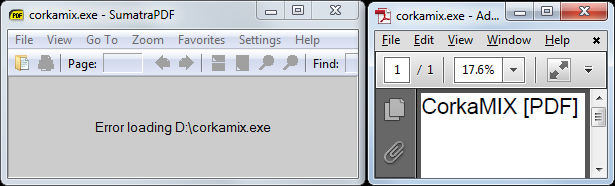
\includegraphics[width=0.8\textwidth]{albertini/img/undocumentedPDF}
  \caption{notre PDF documenté n'est pas géré par un lecteur plus rigoureux qu'Acrobat}
  \label{fig:albertini:undocumentedPDF}
\end{figure}


\subsection{une structure ZIP incorrecte}

Java ne prend pas en compte les CRCs du format ZIP, ne pas les générer nous donne un ZIP à priori invalide mais parfaitement fonctionnel via Java
\begin{figure}[ht]
  \centering
  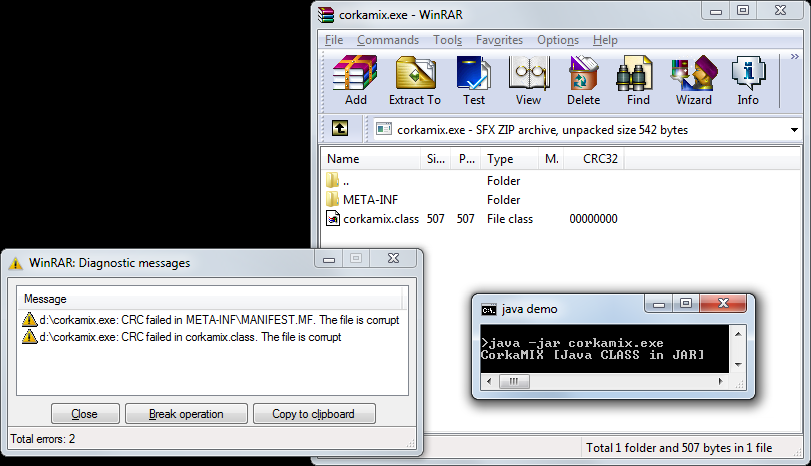
\includegraphics[width=0.8\textwidth]{albertini/img/wrong_crcs}
  \caption{Java passe outre les CRCs invalides}
  \label{fig:albertini:wrong_crcs}
\end{figure}

\subsection{mélangeons le tout}
on peut donc concaténer chaque structure.

par exemple, la partie principale du PDF sera intégré à la classe Java, dans sa {\em ConstantPool}.

\begin{figure}[ht]
  \centering
  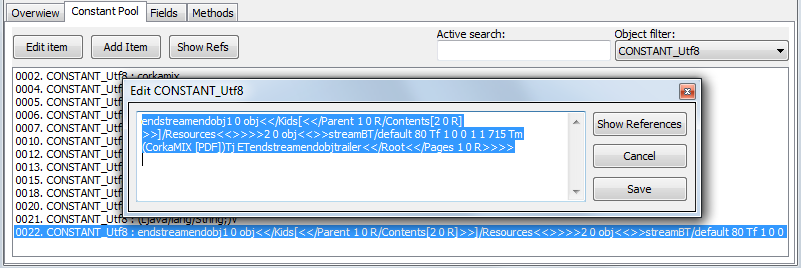
\includegraphics[width=0.8\textwidth]{albertini/img/pdfpool}
  \caption{une classe Java contenant du PDF}
  \label{fig:albertini:pdfpool}
\end{figure}

\subsection{un patchwork binaire}
\begin{figure}[ht]
  \centering
  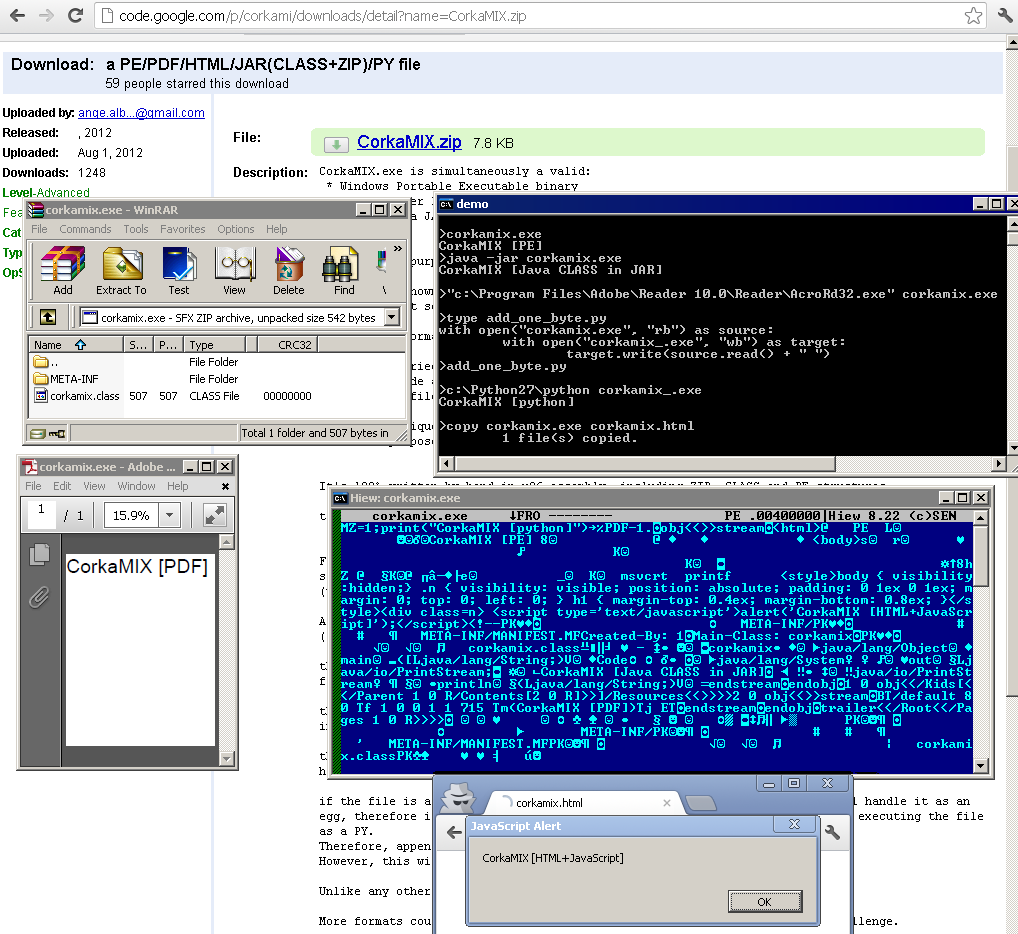
\includegraphics[width=0.8\textwidth]{albertini/img/corkamix}
  \caption{un joli patchwork}
  \label{fig:albertini:corkamix}
\end{figure}

Signature initiale: PE

récapitulons tous les formats inclus:
\begin{itemize}
\item[exécutable] PE
\item[exécutable] Java
\item[script] python (si le Java est désactivé)
\item[script] JavaScript
\item[document] PDF
\item[archive] ZIP
\item[document] HTML
\end{itemize}

on peut rajouter de nombreux formats dans le fichier Zip lui-même, mais ça ne présente aucun challenge particulier.

ça pose donc beaucoup de problèmes - VirusTotal ne l'identifie que comme PDF.
\begin{figure}[ht]
  \centering
  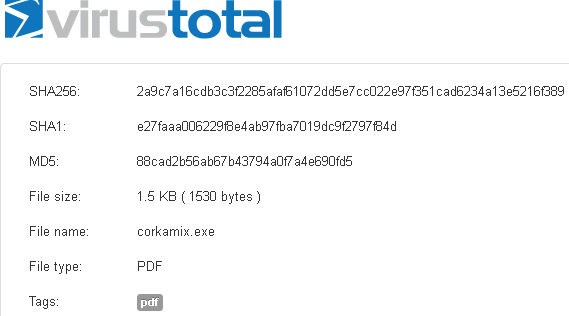
\includegraphics[width=0.8\textwidth]{albertini/img/corkamix-vt}
  \caption{un exécutable identifié uniquement comme PDF}
  \label{fig:albertini:corkamix-vt}
\end{figure}

\subsection{autres systèmes d'exploitations}

Un esprit moqueur serait tenté de se contenter de blamer Microsoft et Adobe pour leur laxisme, et d'accepter ainsi n'importe quel format binaire.

\subsubsection{Linux}

En regardant le format PDF dans un premier temps, on s'aperçoit que les visualisateurs PDF standard sous Linux, bien que n'acceptant pas le PDF particulier généré précedemment, n'en sont pas pour autant très rigoureux.

En effet, en creusant un peu, on s'aperçoit que de nombreux outils PDF tels qu'Evince ou l'outil standard d'Ubuntu, acceptent un PDF ne contenant même pas une signature $\%PDF$, meme partielle,ce qu'Adobe Reader refusera immediatement.

le format binaire Linux, {\it Executable File Format}, n'impose rien de particulier concernant le fichier lui-meme. Creer un tel polyglotte basé sur un ELF plutot qu'un PE ne présente alors pas de difficulté particuliere.

\begin{figure}[ht]
  \centering
  \includegraphics[width=0.8\textwidth]{albertini/img/corkaminux}
  \caption{un polyglotte binaire sous Linux}
  \label{fig:albertini:corkaminux}
\end{figure}

\subsubsection{OS X}

Les visualisateurs standards OS X et iOS sont eux, beaucoup plus stricts.

Ils refusent toute signature incomplete ou absente. Les seules malformations théoriques acceptées sont l'absence de $xref$, longueurs de flux ($stream /length$), et signature de fin de fichier $\%EOF$.

Le format binaire d'OS X, le Mach-O (pour Mach Object) ne présente pas, à l'instar du format ELF, aucune difficulté particulière une fois qu'on en a la maitrise de leur structure binaire.
\begin{figure}[ht]
  \centering
  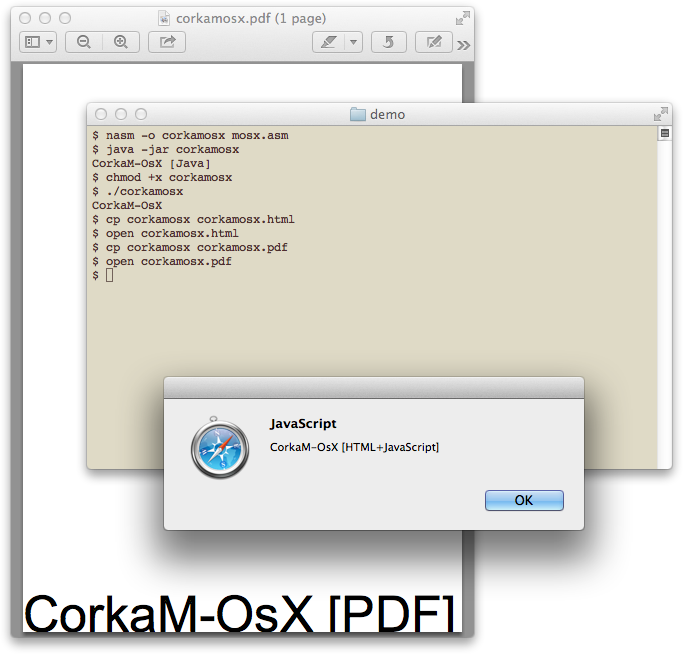
\includegraphics[width=0.8\textwidth]{albertini/img/corkamosx}
  \caption{un polyglotte binaire sous OS X}
  \label{fig:albertini:corkamosx}
\end{figure}


\section{conséquences pour la sécurité}
Tels des marques de lessives, les outils de sécurité sont comparés selon de trop simples critères: vitesse d'analyse et taux de détection d'un même ensemble empirique d'exécutables.

Tout outil d'analyse commercial grand-public a donc la lourde responsabilité de ne pas trop s'attarder sur un fichier particulier. En conséquence, il est crucial que le moteur de celui-ci détecte au plus tôt, et efficacement, le type du fichier analysé.

On peut donc imaginer le début de l'exécution d'un tel outil comme une grosse gare de triage: il n'est donc pas surprenant qu'un fichier, une fois détecté comme un seul type de format (comme le montre la figure \ref{fig:albertini:corkamix-vt}), sera analysé comme tel, et donc ne sera pas réanalysé par la suite comme étant d'un autre format.

Quand bien même il le serait, l'outil ne vas pouvoir se permettre de réanalyser totalement le fichier comme étant d'un autre format, car il va au bout d'un moment couper l'analyse, pour ne pas s'attarder trop longtemps sur un fichier unique.

Une première démarche est donc de légitimement feindre un format de fichier, faisant que l'outil ciblé analysera se fichier comme tel, puis, ne trouvant rien de malveillant dans ce format particulier, déclarera le fichier comme sain.
Ça peut donc se faire simplement en commençant un fichier par la signature {\em PE},
puis en continuant le fichier comme un fichier {\em HTML} ou {\em PDF}.

Une deuxième démarche consiste à inclure un maximum de format, pour que, quelque soit l'ordre d'analyse de l'outil, il atteigne sa limite imposée de temps/cycles, et ainsi qu'il abandonne avant d'avoir pu déterminer si le fichier est sain ou non.

Une autre possibilité est que le fichier cause des problèmes au moteur de l'outil, et qu'il échoue directement.

La première priorité pour l'outil est de déterminer au plus tôt qu'il y a une combinaison inhabituelle de formats binaires dans un seul fichier, ce qui augmente la suspicion. Si cette combinaison ne concerne aucun cas légitime, le fichier peut être classé comme malveillant selon cet unique critère. Malheureusement, cette combinaisons de formats peut être perçue comme un avantage technique par des développeurs peu renseignés, et, bien que déconseillée en pratique, peut être rencontrée dans la nature.

D'autre part, tous les navigateurs modernes analysent l'intégralité d'un fichier pour son contenu Web, même s'il est hors norme: par exemple, un fichier constitué d'un exécutable {\em PE} de $27 Mo$ suivi d'une page Web fonctionnera toujours dans les 2 formats. Un outil de sécurité grand public se devra de se limiter {\it à priori} aux premiers méga-octets, pour optimiser sa performance.

\begin{figure}[ht]
  \centering
  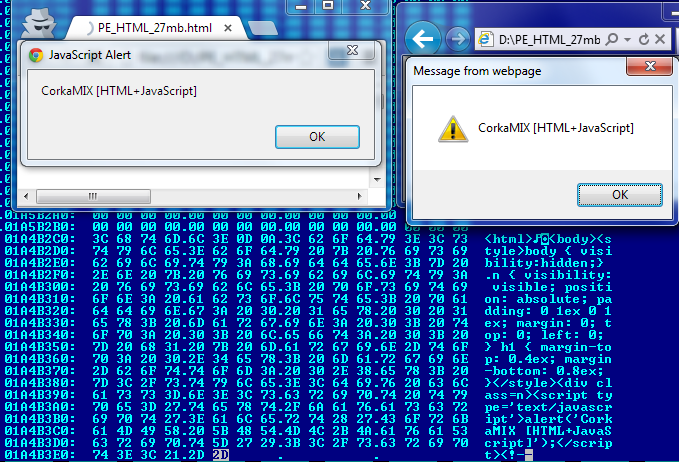
\includegraphics[width=0.8\textwidth]{albertini/img/PE_HTML_27mb}
  \caption{une page HTML à la suite d'un PE de 27Mo}
  \label{fig:albertini:PE_HTML_27mb}
\end{figure}

\section{conclusion}
Après avoir vu que la combinaisons de formats binaires dans un seul fichier et possible, et vu en détail ses conséquences possibles sur la détection de code malveillant, on voit donc que ce mélange possible de formats binaires ne simplifie pas du tout l'analyse automatisée - voire même manuelle - de fichiers binaires, et complique bien la tâche.

Il semble donc indispensable de ne créer que des standards déterminés par une signature unique au début du fichier.

Il ne semble pas déraisonnable d'aller plus loin, et de rejeter tout nouveau format de fichier conçu autrement.
\bibliography{albertini/biblio}

%%% Local Variables:
%%% mode: TeX-PDF
%%% TeX-master: "master"
%%% End:
